\documentclass[pdflatex,11pt]{../aghdoc_version2}
%\documentclass{../aghdoc}               % przy kompilacji programem latex
\usepackage[polish]{babel}
\usepackage[utf8]{inputenc}

% dodatkowe pakiety
\usepackage[hidelinks]{hyperref}
\usepackage{enumerate}
\usepackage{listings}
\usepackage{caption}

% żeby stopki były zastosowane do stron gdzie rozpoczyna się rozdział
\usepackage{etoolbox}
\patchcmd{\chapter}{\thispagestyle{plain}}{\thispagestyle{fancy}}{}{}

\lstloadlanguages{TeX}

\lstset{
  literate={ą}{{\k{a}}}1
           {ć}{{\'c}}1
           {ę}{{\k{e}}}1
           {ó}{{\'o}}1
           {ń}{{\'n}}1
           {ł}{{\l{}}}1
           {ś}{{\'s}}1
           {ź}{{\'z}}1
           {ż}{{\.z}}1
           {Ą}{{\k{A}}}1
           {Ć}{{\'C}}1
           {Ę}{{\k{E}}}1
           {Ó}{{\'O}}1
           {Ń}{{\'N}}1
           {Ł}{{\L{}}}1
           {Ś}{{\'S}}1
           {Ź}{{\'Z}}1
           {Ż}{{\.Z}}1
}

%---------------------------------------------------------------------------

\author{Tomasz Kasprzyk, Daniel Ogiela, Jakub Stępak}
\shortauthor{T. Kasprzyk, D. Ogiela, J.Stępak}

\titlePL{System obliczający wyniki wyborów dla uogólnienia systemu k-Borda}

\shorttitlePL{System obliczający wyniki wyborów dla uogólnienia systemu k-Borda} % skrócona wersja tytułu jeśli jest bardzo długi

\thesistypePL{Dokumentacja użytkownika}

\supervisorPL{dr hab. inż. Piotr Faliszewski}

\date{2016}

\departmentPL{Katedra Informatyki}

\facultyPL{Wydział Informatyki, Elektroniki i Telekomunikacji}

\setlength{\cftsecnumwidth}{10mm}

% umożliwienie żeby domyślnie dokument nie robił wcięć poza wybranymi (\indent w tym miejscu)

\newlength\tindent
\setlength{\tindent}{\parindent}
\setlength{\parindent}{0pt}
\renewcommand{\indent}{\hspace*{\tindent}}

\fancypagestyle{plain}{%
\fancyhf{} % clear all header and footer fields
\fancyhead[R]{\bfseries \thepage}
\fancyfoot[C]{System obliczający wyniki wyborów dla uogólnienia systemu k-Borda} % except the center
\renewcommand{\headrulewidth}{0.5pt}
\renewcommand{\footrulewidth}{0.5pt}}

%---------------------------------------------------------------------------

\begin{document}

\titlepages

\tableofcontents

%----------------------------------------------------------------------------
\chapter{Wstęp}
\label{cha:wstep}

Niniejszy podręcznik opisuje sposób użytkowania systemu \texttt{Election Computing System}, powstałego w ramach pracy inżynierskiej realizowanej na Akademii Górniczo-Hutniczej w Krakowie.

System umożliwia obliczenie wyników wyborów w uogólnionym systemie wyborczym k-Borda.

Szczegóły na temat tego systemu wyborczego można przeczytać w Przewodniku po projekcie.


\chapter{Instrukcja uruchomienia systemu}
\label{cha:uruchomienie}

Działającą aplikację można przetestować na stronie: \\ \url{https://election-computing-system.herokuapp.com}. 

Ze względu na ograniczenia na liczbę rekordów w bazie danych narzucone przez darmową wersję Heroku, nie będzie można dodać tam zbyt „dużych” wyborów (ograniczona jest liczba głosujących i kandydatów). Aby korzystać z pełnych możliwości aplikacji, należy uruchomić ją na własnym komputerze. Dalsza część tego rozdziału opisuje jak to wykonać.

\section{Przygotowanie środowiska}
\label{sec:srodowisko}

\subsection{Język}
\label{subsec:jezyk}

System jest aplikacją internetową opartą o framework \textit{Django }napisaną w języku \textit{Python 2.7}.
Aby uruchomić aplikację, należy uprzednio zainstalować na swoim komputerze interpreter \textit{Pythona}.

\subsection{Repozytorium}
\label{subsec:repo}

Repozytorium projektu znajduje się pod adresem: \\ \url{https://github.com/jakubste/election-computing-system}.
Projekt należy sklonować używając programu \textit{Git} 
\begin{lstlisting}[language=bash]
$ git clone git@github.com:jakubste/election-computing-system.git
\end{lstlisting}
lub ściągnąć jako ZIP bezpośrednio z serwsiu \textit{GitHub} i rozpakować w wybranym miejscu.

\subsection{Biblioteki}
\label{subsec:biblioteki}

Do instalacji bibliotek zaleca się używanie mechanizmu \texttt{virtualenv}, który separuje środowiska uruchomieniowe dla poszczególnych projektów. Autorzy projektu zalecają też dla wygody wykorzystanie \texttt{virtualenvwrapper}'a. Do instalacji bibliotek można użyć programu \texttt{pip}.
Informacje o wymaganych bibliotekach są zawarte w pliku \texttt{requirements.txt}.
\begin{lstlisting}[language=bash]
$ mkvirtualenv inz
$ pip install -r requirements.txt
\end{lstlisting}

\subsection{Baza danych}
\label{subsec:database}

Aplikacja domyślnie jest skonfigurowana do użycia z bazą danych dostarczaną przez \textit{Heroku} (\textit{PostreSQL}). Dla ułatwienia zostanie przedstawiony sposób konfiguracji z użyciem \textit{SQLite3}. O konfiguracji dostępu do innych baz danych można przeczytać w dokumentacji \textit{Django}. 

W celu skonfigurowania swojej bazy danych należy w katalogu \texttt{ecs} utworzyć 
plik \texttt{local\_settings.py} i umieścić tam następujący kod:

\begin{lstlisting}[language=Python]
from settings import *

DATABASES = {
   'default': {
       'ENGINE': 'django.db.backends.sqlite3',
       'NAME': os.path.join(BASE_DIR, 'db.sqlite3'),
   }
}
\end{lstlisting}

Następnie w katalogu głównym programu należy wykonać polecenie:
\begin{lstlisting}[language=bash]
$ ./manage.py migrate
\end{lstlisting}


\section{Uruchomienie serwera}
\label{sec:serwer}

W tym momencie aplikacja powinna być gotowa do działania.
W katalogu głównym programu należy wykonać polecenie:
\begin{lstlisting}[language=bash]
$ ./manage.py run_server
\end{lstlisting}

Po otworzeniu w przeglądarce internetowej adresu:
\begin{lstlisting}
http://localhost:8000/
\end{lstlisting}
powinna pojawić się strona podobna do tej: \\ 

%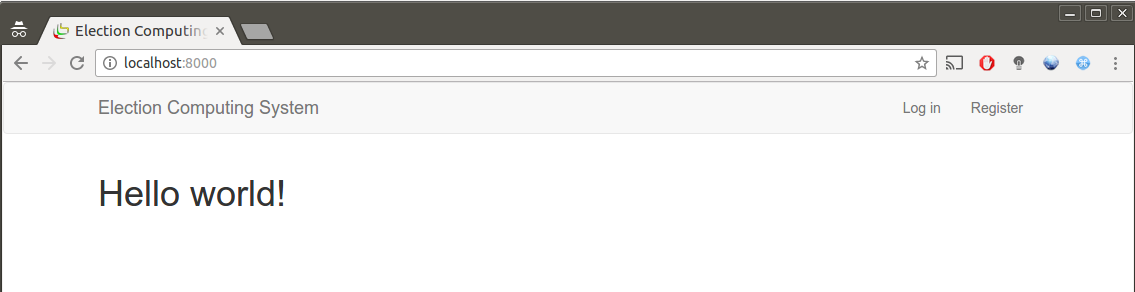
\includegraphics[width=0.8\textwidth]{pics/first_view.png}
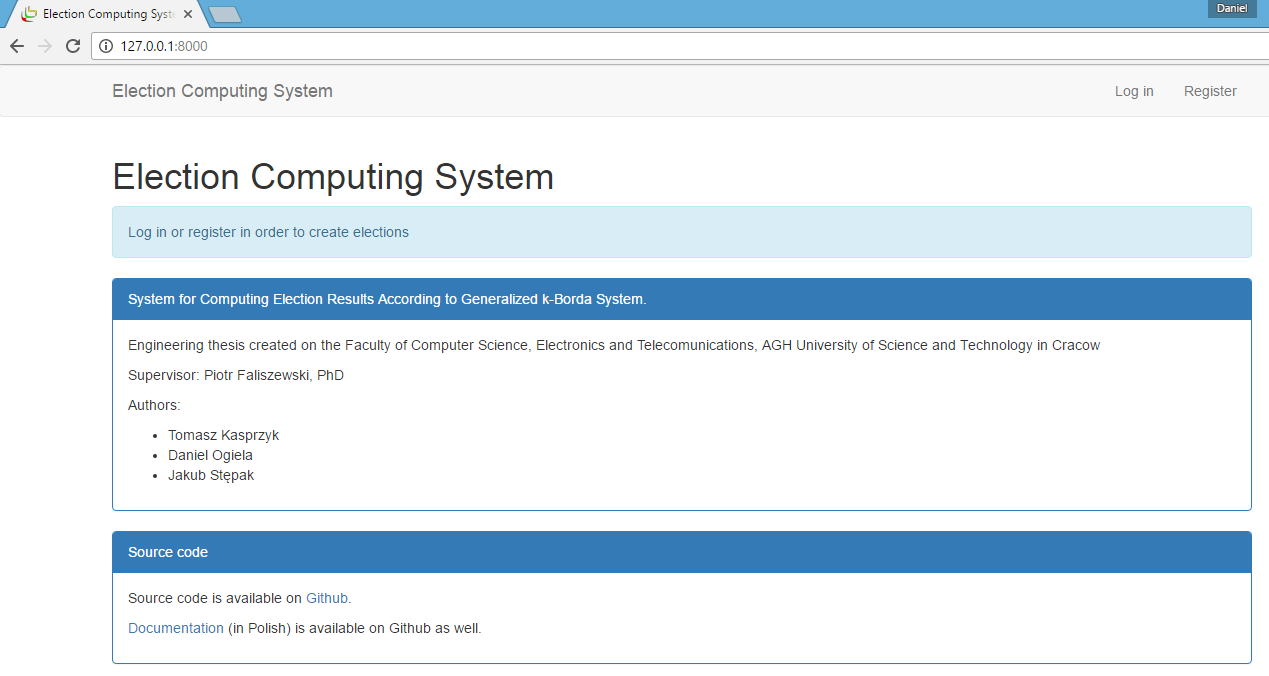
\includegraphics[width=1\textwidth]{pics/first_view_version2.png}
\captionof{figure}{Strona startowa}


\chapter{Instrukcja obsługi systemu}
\label{cha:obsluga}


\section{Rejestracja}
\label{sec:rejestracja}

Aby korzystać z systemu, należy utworzyć konto. W tym celu należy wybrać opcję rejestracji z górnego panelu strony. \\

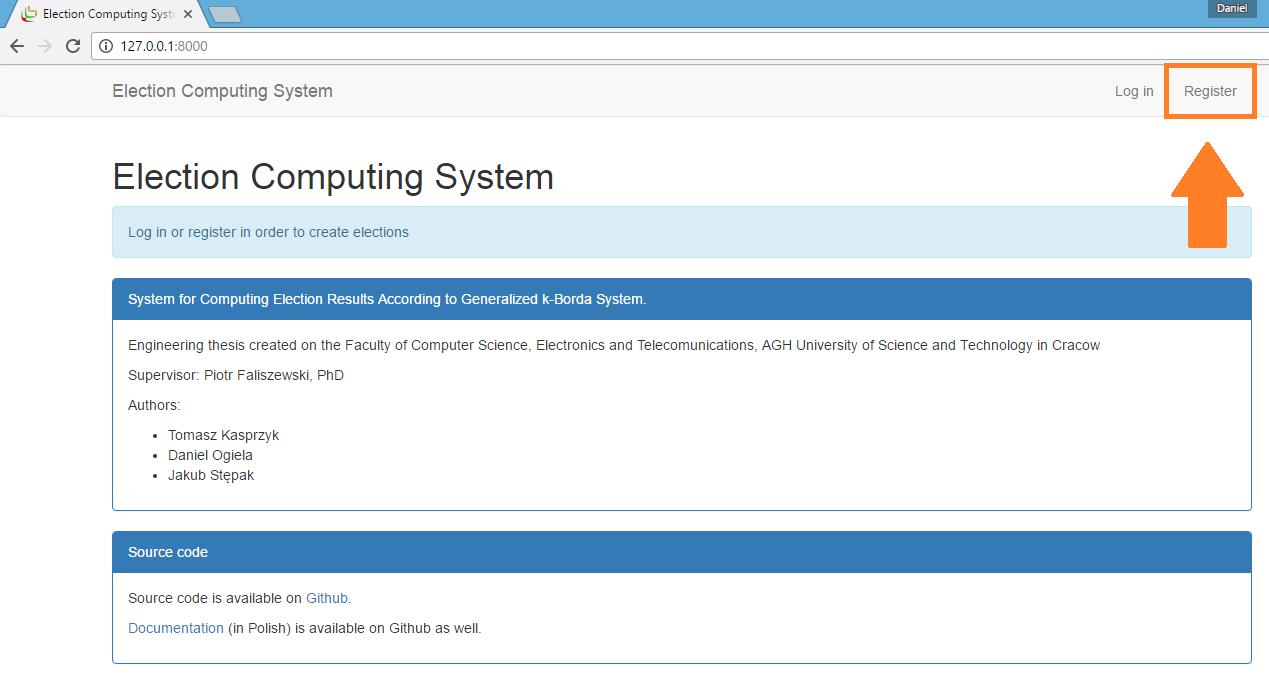
\includegraphics[width=1\textwidth]{pics/registration_button.png}
\captionof{figure}{Przycisk do rejestracji konta}

\vspace{\baselineskip}
\vspace{\baselineskip}
Po naciśnięciu przycisku do rejestracji konta, powinna pojawić się strona z formularzem do uzupełnienia. Kolejne pola poczynając od góry oznaczają odpowiednio: adres e-mail, nazwa użytkownika, hasło, imię oraz nazwisko. Po wypełnieniu formularza należy nacisnąć \textit{Register} znajdujący się pod ostatnim polem formularza. 

\begin{center}
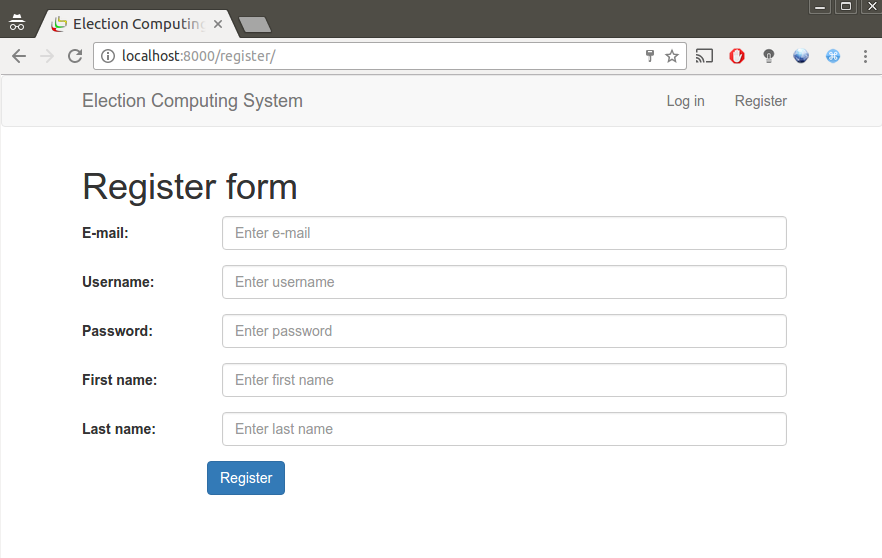
\includegraphics[width=0.8\textwidth]{pics/register.png}
\captionof{figure}{Formularz do rejestracji konta}
\end{center}

%\newpage
\section{Logowanie}
\label{sec:logowanie}

W celu zalogowania się na wcześniej utworzone konto należy wybrać opcję logowania z górnego panelu strony startowej. \\

\begin{center}
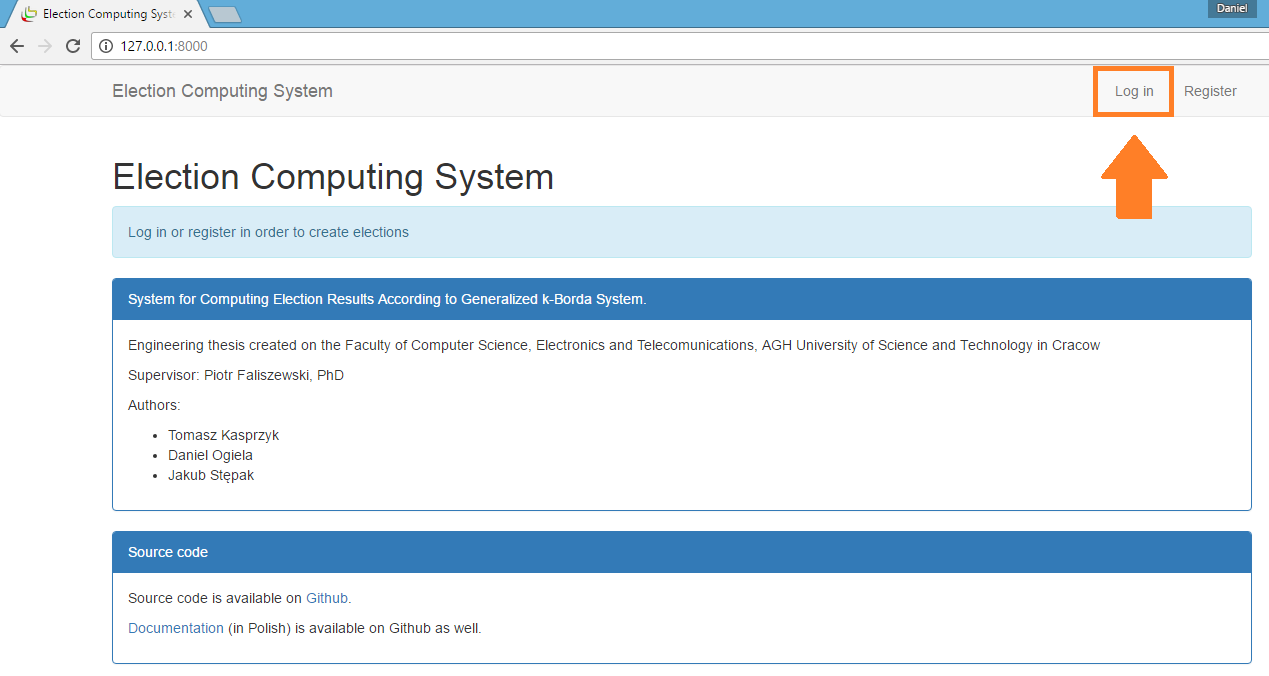
\includegraphics[width=1\textwidth]{pics/login_button.png}
\captionof{figure}{Przycisk do logowania na startowej stronie}
\end{center}

\newpage
Po naciśnięciu przycisku do logowania, powinna pojawić się strona z formularzem do uzupełnienia. Kolejne pola poczynając od góry oznaczają odpowiednio: nazwa użytkownika oraz hasło. Po wypełnieniu formularza zgodnie z danymi dostępu do konta należy nacisnąć \textit{Log in} znajdujący się pod ostatnim polem formularza. \\

\begin{center}
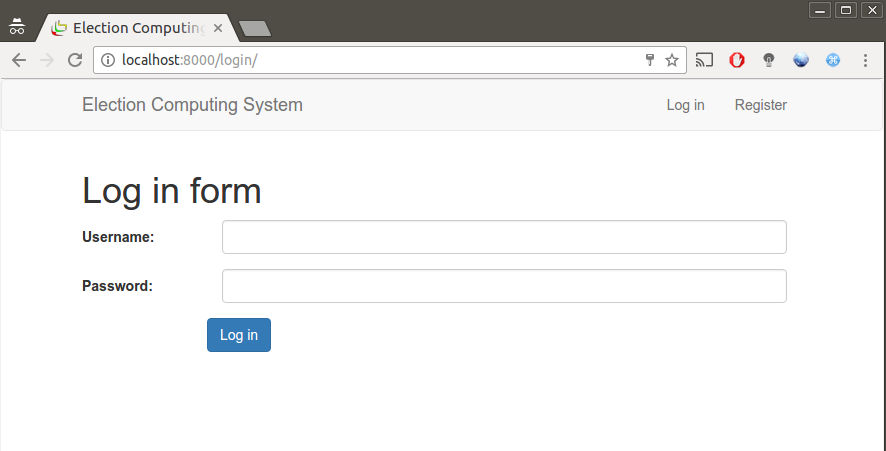
\includegraphics[width=0.8\textwidth]{pics/login.png}
\captionof{figure}{Formularz do zalogowania się na konto}
\end{center}

\section{Strona główna}
\label{sec:stronaglowna}

Po zalogowaniu użytkownik widzi stronę główną z opisem systemu: \\

\begin{center}
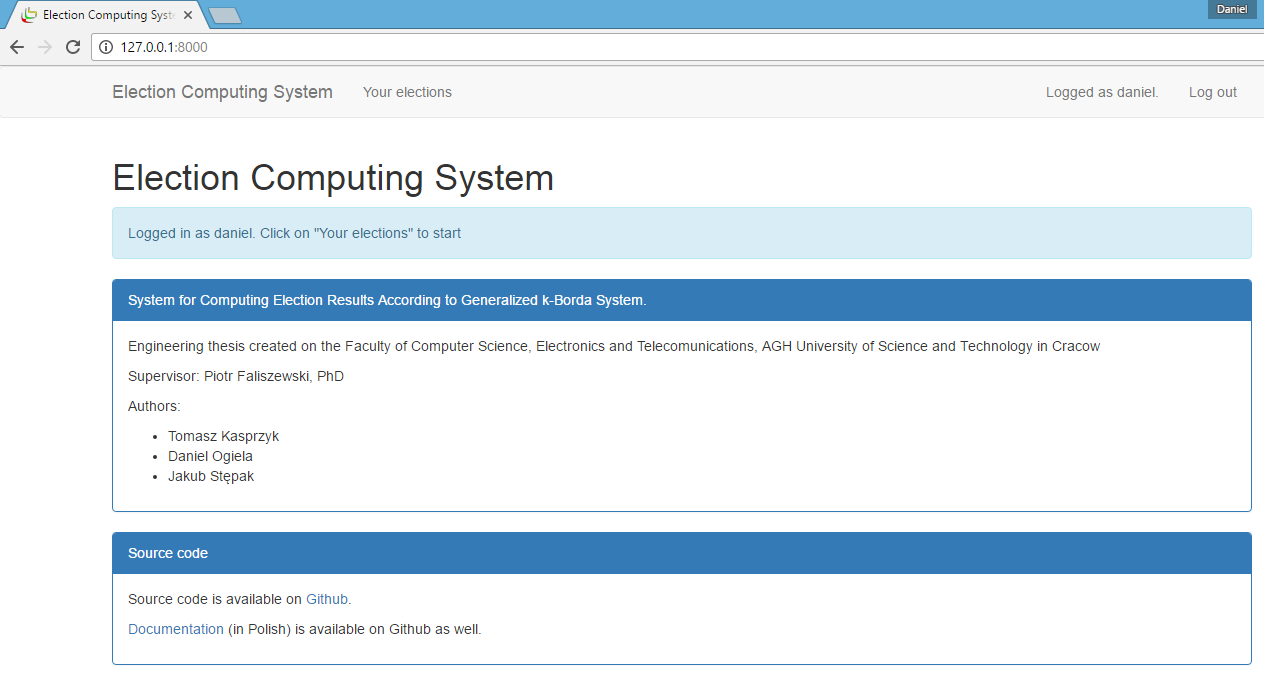
\includegraphics[width=0.8\textwidth]{pics/mainpage_version2.png}
\captionof{figure}{Strona główna systemu po zalogowaniu na konto}
\end{center}

\newpage
\section{Lista wyborów}
\label{sec:electionslist}

W celu wyświetlenia listy zdefiniowanych przez użytkownika wyborów należy nacisnąć przycisk \textit{Your elections} z górnego panelu strony głównej: \\

\begin{center}
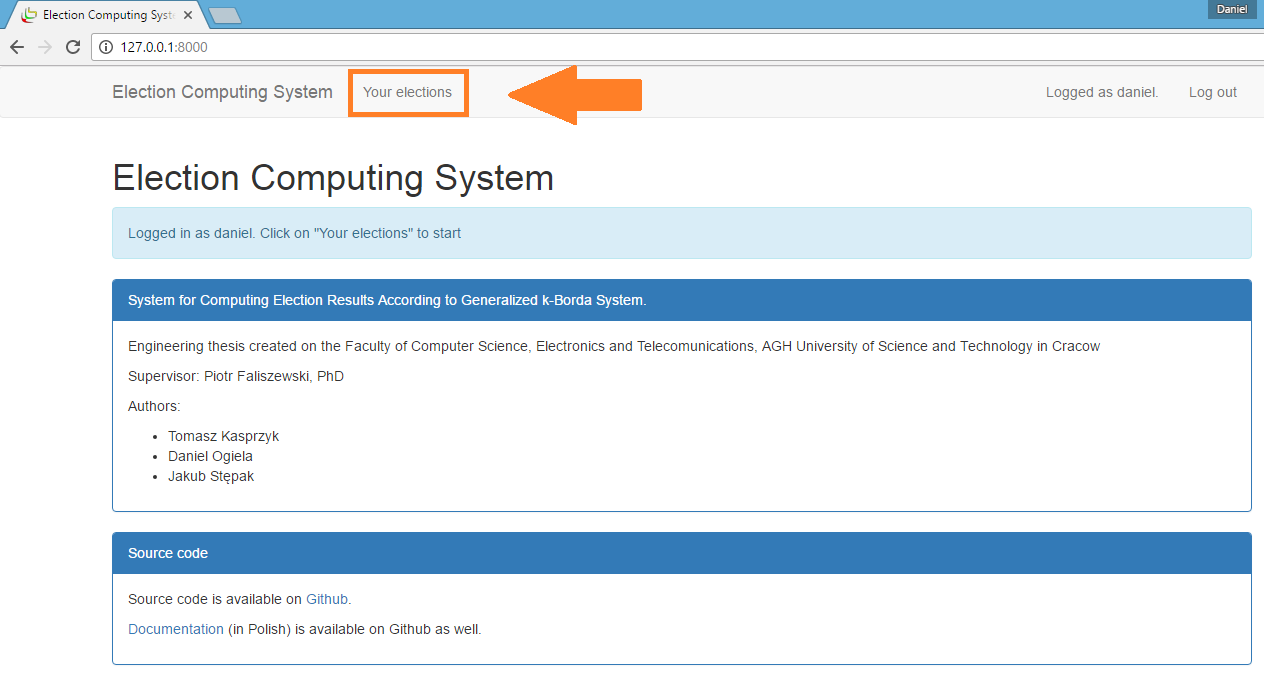
\includegraphics[width=0.8\textwidth]{pics/your_elections_button.png}
\captionof{figure}{Przycisk do wyświetlenia listy wyborów na głównej stronie}
\end{center}

\vspace{\baselineskip}
Po wybraniu z menu odpowiedniego przycisku użytkownik ma możliwość zobaczenia listy swoich wyborów: \\

\begin{center}
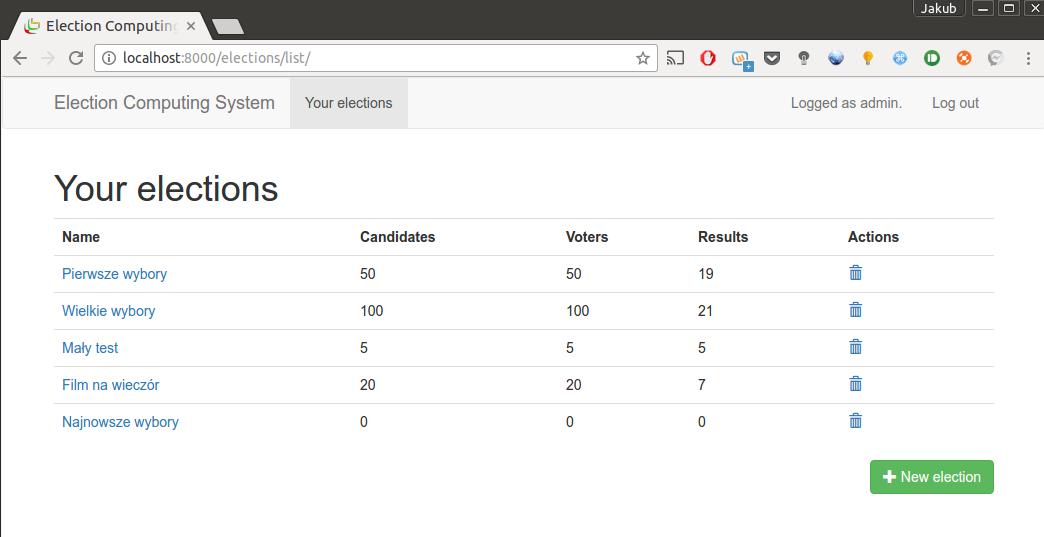
\includegraphics[width=0.8\textwidth]{pics/elections-list.png}
\captionof{figure}{Strona z listą zdefiniowanych wyborów}
\end{center}

Stąd użytkownik ma możliwość przejścia do tworzenia nowych wyborów.


\section{Tworzenie wyborów}
\label{sec:electionscreate}


Aby utworzyć nowe wybory należy nacisnąć przycisk \textit{New election} na stronie z listą zdefiniowanych wyborów: \\

\begin{center}
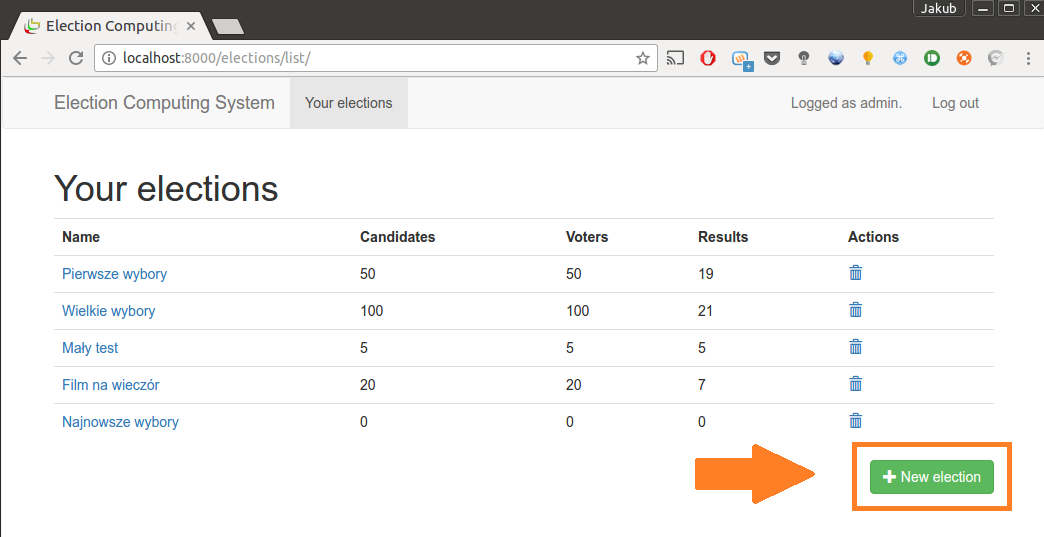
\includegraphics[width=0.8\textwidth]{pics/new_election_button.png}
\captionof{figure}{Przycisk do stworzenia nowych wyborów}
\end{center}

\vspace{\baselineskip}
Po naciśnięciu wskazanego przycisku powinna pojawić się strona z formularzem. Należy w nim podać nazwę wyborów oraz określić rozmiar komitetu, dla którego przeprowadzamy wybory. Po wypełnieniu formularzu należy nacisnąć przycisk \textit{Create election} znajdujący się pod ostatnim polem formularza: \\

\begin{center}
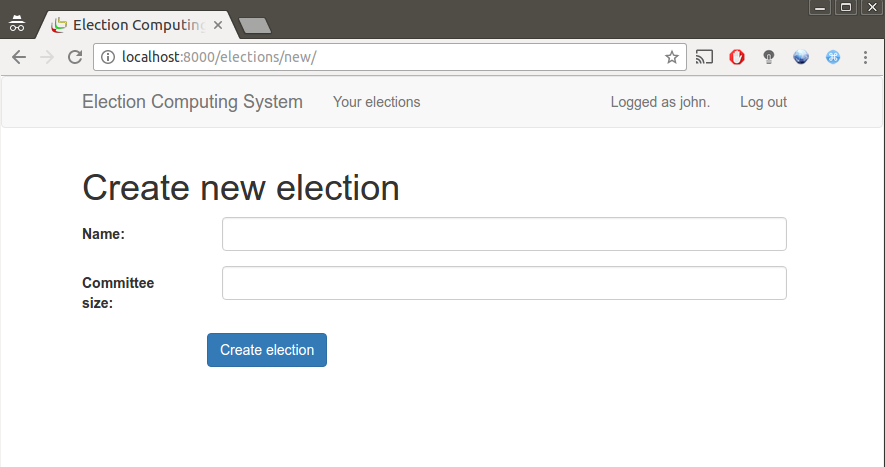
\includegraphics[width=0.8\textwidth]{pics/elections-new.png}
\captionof{figure}{Formularz do zdefiniowania wyborów}
\end{center}

\newpage
\section{Określenie kandydatów i wyborców}
\label{sec:electionsnewlycreated}

Po utworzeniu wyborów należy określić biorących udział w wyborach kandydatów oraz wyborców.
Użytkownik ma do wyboru dwie opcje:
\begin{itemize}
\item wczytać dane z pliku w formacie .soc określonym przez \href{http://www.preflib.org/}{PrefLib},
\item wygenerować losowy układ wyborców w oparciu o rozkład normalny.
\end{itemize}


\subsection{Wczytanie danych z pliku}
\label{subsec:wczytaniezpliku}

Aby wczytać dane dotyczące wyborów z pliku, należy wybrać odpowiednią opcję na stronie z wyborami, która wyświetla się po stworzeniu wyborów: \\

\begin{center}
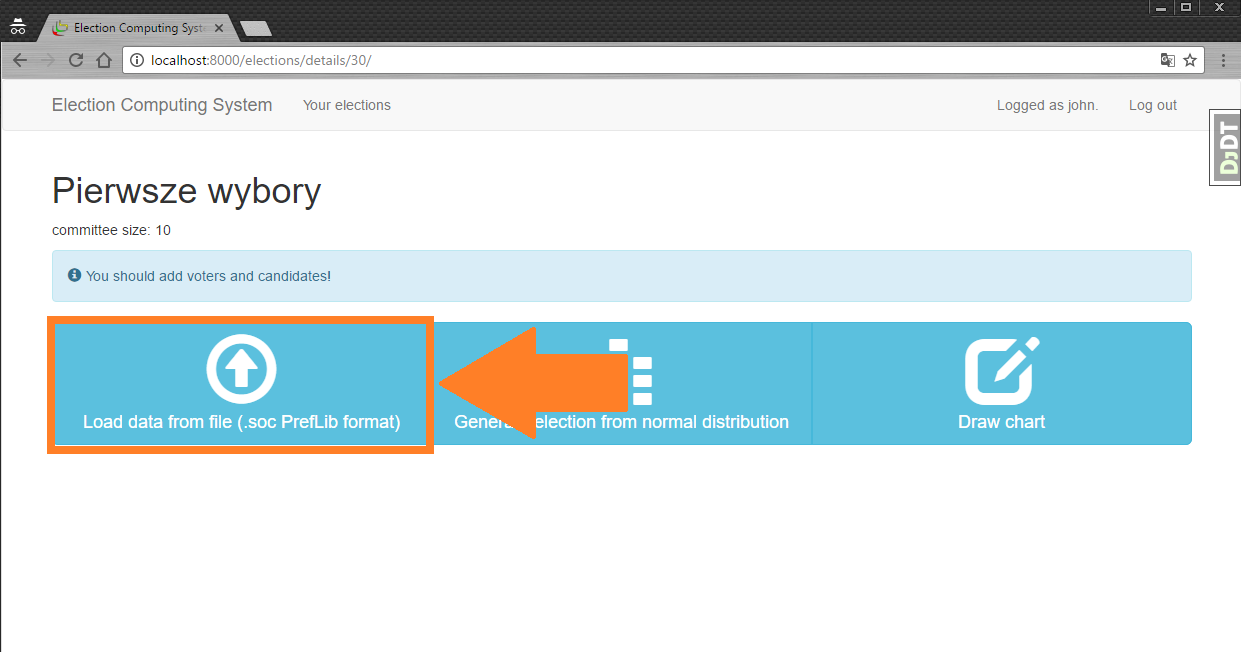
\includegraphics[width=0.8\textwidth]{pics/load_data_from_file_button.png}
\captionof{figure}{Przycisk do wczytania danych z pliku na stronie z wyborami}
\end{center}


\vspace{\baselineskip}
\vspace{\baselineskip}
\vspace{\baselineskip}
Po wyborze odpowiedniej opcji, należy wcisnąć przycisk \textit{Wybierz plik} na wyświetlonej stronie, wskazać plik z danymi w systemie plików, a na końcu potwierdzić wybór przyciskiem \textit{Load data} znajdujący się pod polem z nazwą wskazanego pliku: 

\newpage

\begin{center}
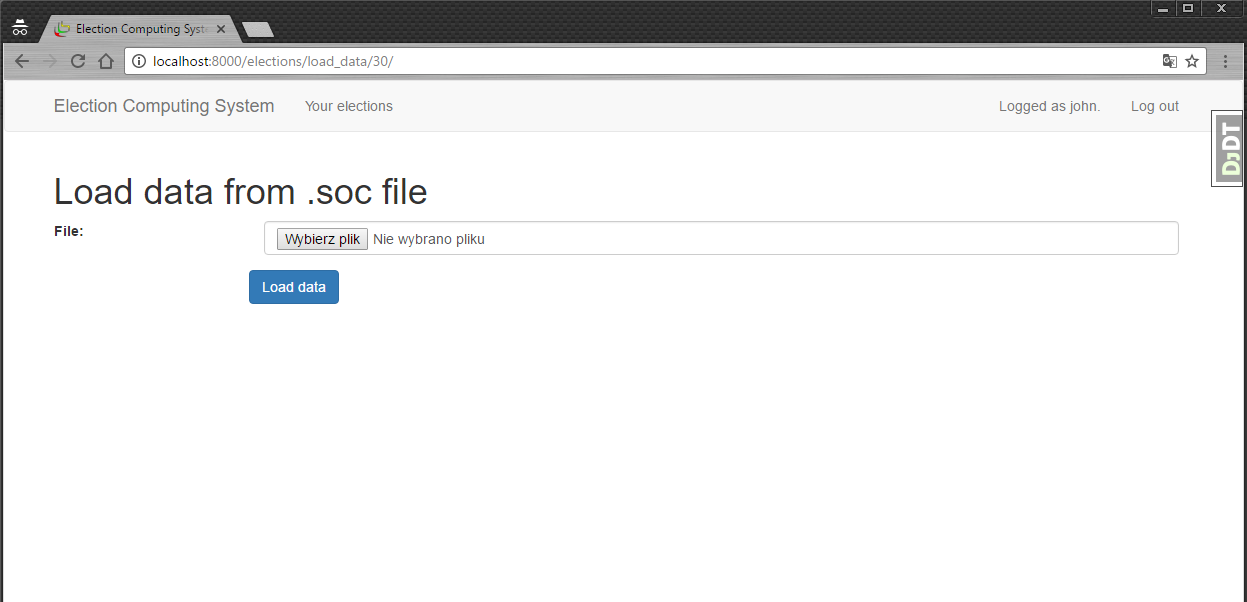
\includegraphics[width=0.8\textwidth]{pics/load-from-file.png}
\captionof{figure}{Strona do wskazania pliku z danymi}
\end{center}

Przykładowe pliki z danymi można pobrać ze strony projektu \href{http://www.preflib.org/data/packs/index.php#soc}{PrefLib}. Pośród tych plików można m.in. znaleźć rzeczywiste preferencje studentów naszego kierunku w wyborach przedmiotów obieralnych.

\subsection{Generacja danych z rozkładu normalnego}
\label{subsec:generowaniedanych}

Aby wygenerować dane losowe na podstawie rozkładu normalnego należy wybrać odpowiednią opcję na stronie z wyborami, która wyświetla się po stworzeniu wyborów: \\

\begin{center}
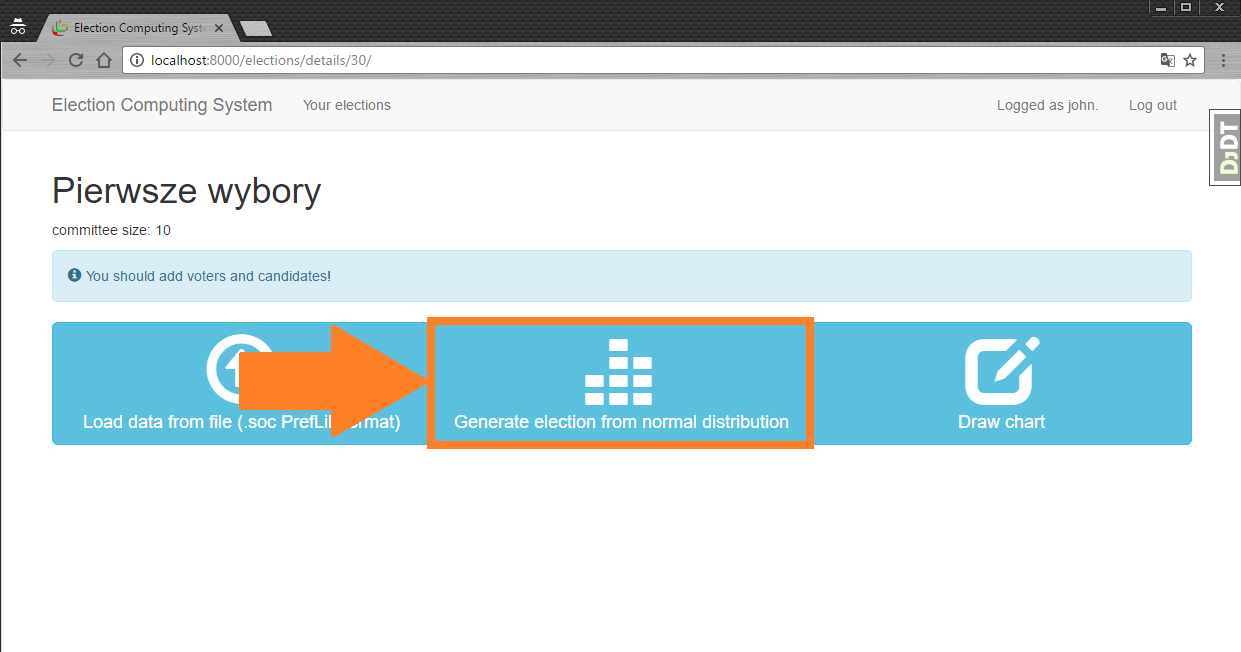
\includegraphics[width=0.8\textwidth]{pics/generate_election_button.png}
\captionof{figure}{Przycisk do wygenerowania danych z rozkładu normalnego}
\end{center}

\newpage
Po wybraniu odpowiedniej opcji, powinna wyświetlić się strona z formularzem do uzupełnienia: \\

\begin{center}
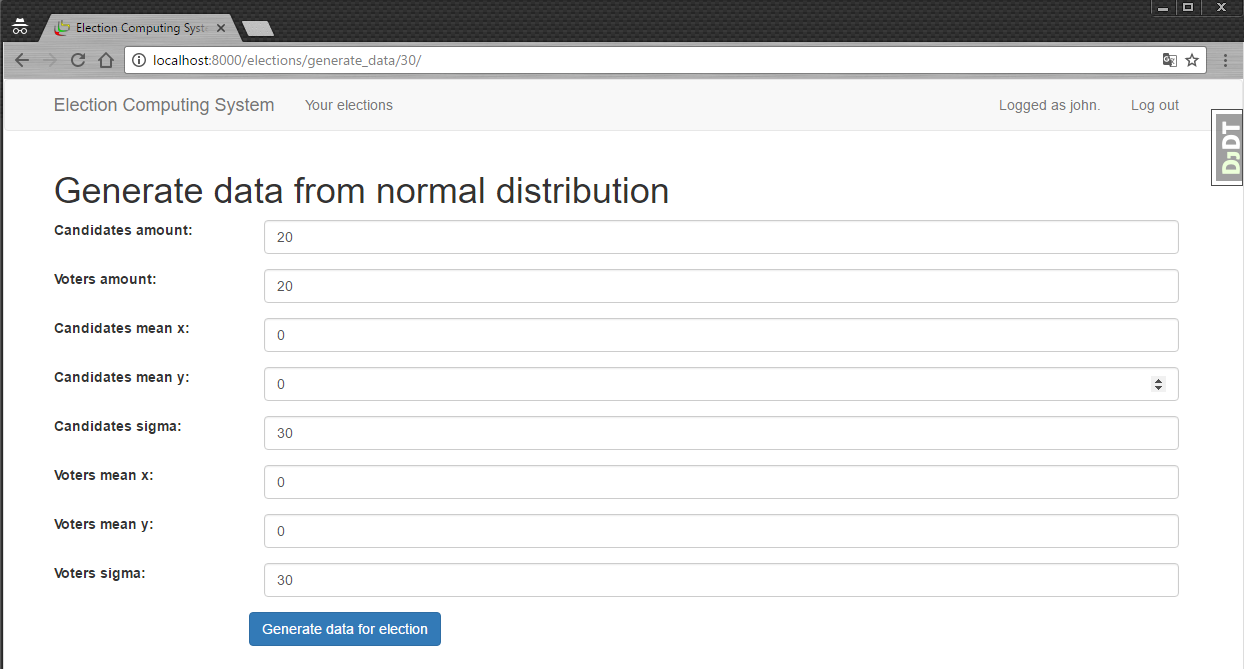
\includegraphics[width=1.0\textwidth]{pics/generate-distribution.png}
\captionof{figure}{Strona z formularzem do wyboru parametrów rozkładu normalnego}
\end{center}

\vspace{\baselineskip}
Kolejne pola formularza począwszy od góry oznaczają odpowiednio: liczbę kandydatów, liczbę wyborców, średnią wartość współrzędnej \textit{x} kandydatów na płaszczyźnie, średnią wartość współrzędnej \textit{y} kandydatów na płaszczyźnie, odchylenie standardowe kandydatów, średnią wartość współrzędnej \textit{x} wyborców na płaszczyźnie, średnią wartość współrzędnej \textit{y} wyborców na płaszczyźnie oraz odchylenie standardowe wyborców.

Średnie określone dla wyborców i kandydatów wyznaczają punkt centralny, wokół którego będą skupione ich „poglądy”.  Odchylenia standardowe określone dla wyborców i kandydatów wyznaczają „stopień rozproszenia poglądów”.

Koncepcyjnie ten sposób generacji danych odzwierciedla mapę poglądów politycznych. Porządek preferencji kandydatów wśród wyborców określa ich odległość euklidesowa w układzie współrzędnych.

Po uzupełnieniu formularza należy potwierdzić wybór przyciskiem \textit{Generate data for election} znajdującym się pod ostatnim polem formularza.

\newpage
\subsection{Rysowanie własnego wykresu}
\label{subsec:wlasnywykres}
Ostatnim z trzech dostępnych sposobów tworzenia wyborów jest ręczne tworzenie wykresu kandydatów i wyborców.

\begin{center}

\includegraphics[width=1.0\textwidth]{pics/paint_election_button.png}
\captionof{figure}{Przycisk otwierający stronę do rysowania własnego wykresu}
\end{center}
Obszar do zaznaczania punktów pokryty jest pomocniczą siatką, podobną jak na wykresach powstałych po
wygenerowaniu punktów zgodnie z rozkładem normalnym. Użytkownik może zaznaczyć na wykresie ograniczoną 
liczbę punktów dla kandydatów i głosujących. Limit określony jest w oknie pomocniczym znajdującym się 
pod obszarem do zaznaczania punktów.\\
Dostępne są dwa tryby kursora - zaznaczanie wyborców oraz zaznaczanie kandydatów. Rozmiar kursora 
początkowo ustawiony jest domyślnie na ``1'' w trybie zaznaczania wyborców.\\
Przełączanie pomiędzy dwoma dostępnymi trybami kursora dostępne jest pod klawiszami ``V'' (\textit{voters}) oraz ``C'' (\textit{candidates}).\\
O tym w jakim trybie pracuje kursor sygnalizuje kolor (niebieski dla głosujacych, zielony dla wyborców) oraz informacja w oknie pod wykresem (Ostatni element na liście - \textit{Adding: \ldots} )

\begin{center}
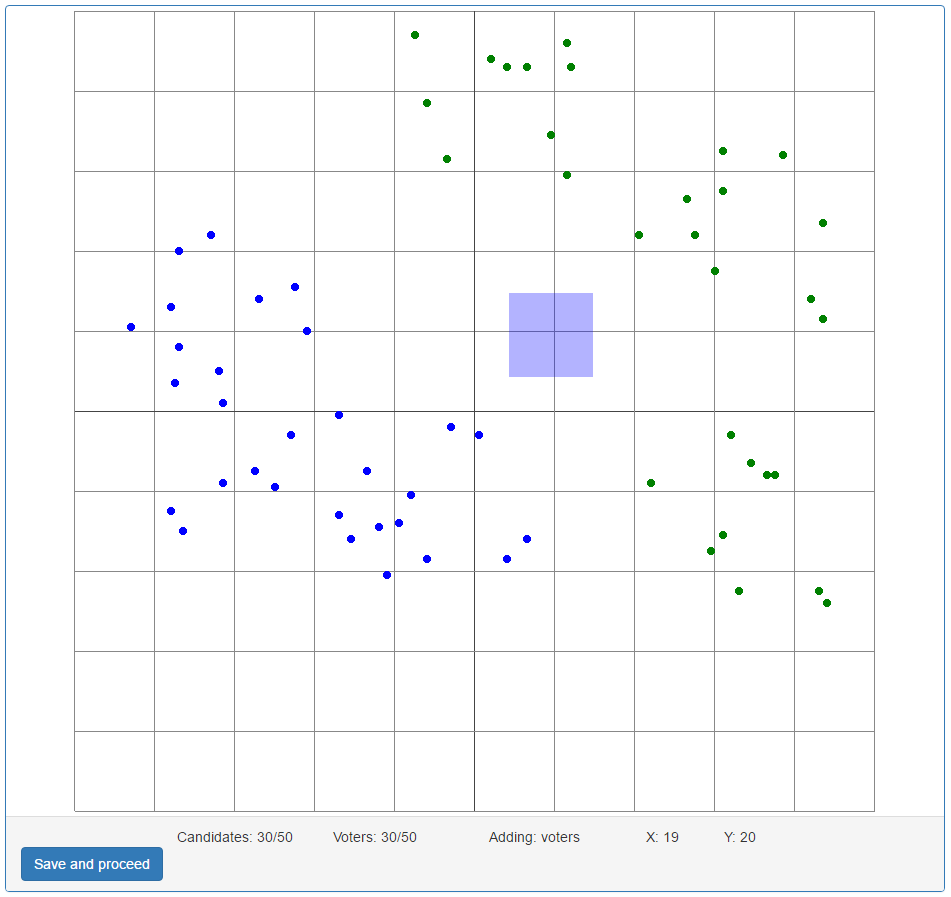
\includegraphics[width=1.0\textwidth]{pics/paint_2.png}
\captionof{figure}{Fragment strony do rysowania wykresu.}
Poniżej wykresu znajduje się krótka instrukcja obsługi edytora oraz przycisk do zapisania 
\mbox{wykresu i przejścia} do szczegółów wyborów
\mbox{\textit{Save and proceed}}
\end{center}

\newpage
Przy użyciu klawiszy ``+'' oraz ``-'' można zmieniać rozmiar kursora. 
Powiększenie kursora skutkuje wygenerowaniem większej liczby punktów przy kliknięciu.
Punkty generowane są losowo, wewnątrz obszaru wyznaczonego przez półprzezroczysty obszar kursora, 
w liczbie proporcjonalnej do wymiarów wspomnianego obszaru.

\begin{center}
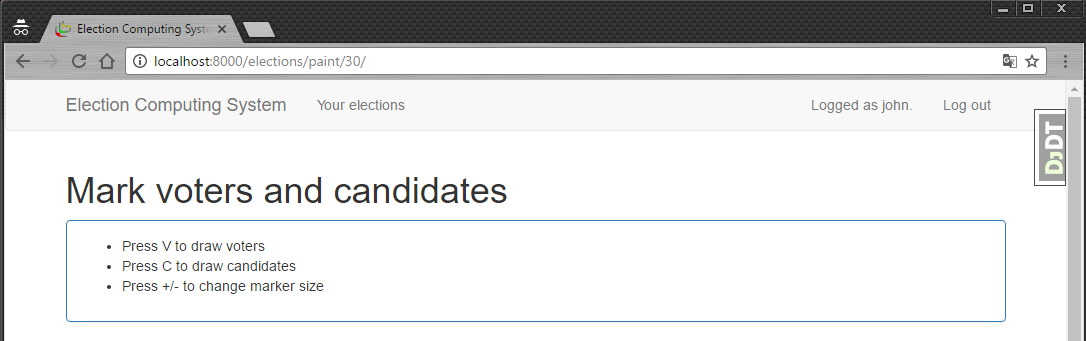
\includegraphics[width=1.0\textwidth]{pics/paint_1.png}
\captionof{figure}{Obszar do zaznaczania współrzędnych kandydatów i wyborców.} Na powyższym rysunku 
kursor ustawiony jest w trybie zaznaczania kandydatów
\end{center}


\newpage
\section{Szczegóły wyborów}
\label{sec:szczegolywyborow}

Po wczytaniu danych pokaże się ekran z szczegółami wyborów: \\
\begin{center}
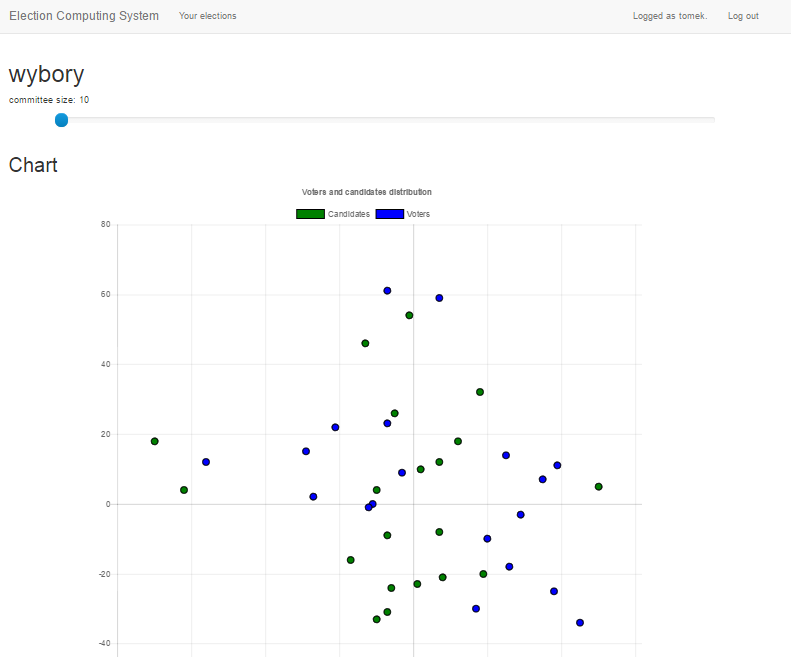
\includegraphics[width=0.8\textwidth]{pics/newlycreated_version2.png}
\captionof{figure}{Strona ze szczegółami wyborów}
\end{center}

\vspace{\baselineskip}
Wykres będzie widoczny tylko w przypadku wyborów wygenerowanych z rozkładu normalnego.

Poniżej można zobaczyć spis dostępnych rozstrzygnięć wyborów, wykres porównujący wyniki wyborów oraz odnośnik do formularza dodawania nowego wyniku.

Poniżej, jeśli liczba wyborców nie jest na tyle duża, że utrudniałoby to używanie strony przez zbytnie obciążenie przeglądarki, widać listing preferencji wyborców. Szczególnie przydatny do sprawdzenia czy poprawnie zostały wczytane dane z plików .soc. W przypadku danych z rozkładu normalnego jego przydatność jest ograniczona.

\newpage
\section{Dodawanie wyniku}
\label{sec:dodawaniewyniku}

W celu dodania wyniku do danych wyborów należy na stronie ze szczegółami wyborów nacisnąć przycisk \textit{Add new result} znajdujący się między panelami z dostępnymi wynikami wyborów (\textit{Available results}) oraz z listingiem preferencji wyborców (\textit{Voters listing}): \\
\begin{center}
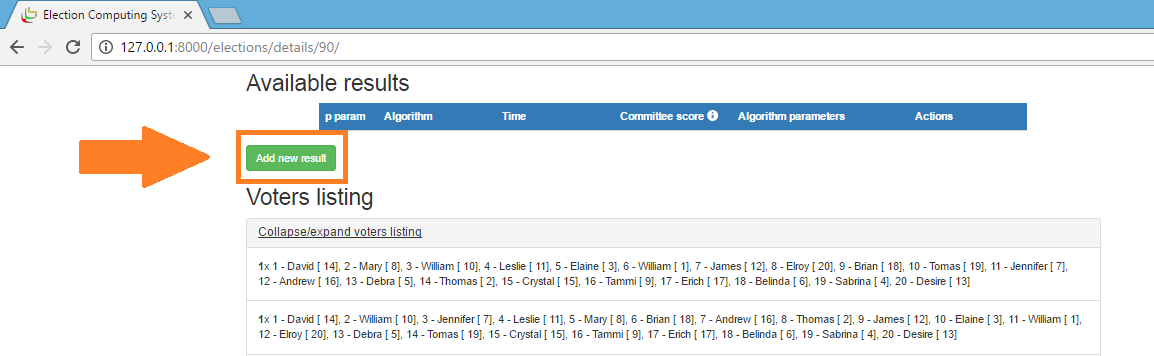
\includegraphics[width=0.8\textwidth]{pics/add_new_result_button.png}
\captionof{figure}{Przycisk do dodania wyniku wyborów na stronie ze szczegółami wyborów}
\end{center}

\vspace{\baselineskip}
Po naciśnięciu odpowiedniego przycisku pojawi się strona z formularzem do określenia parametrów do obliczania wyników wyborów: \\
\begin{center}
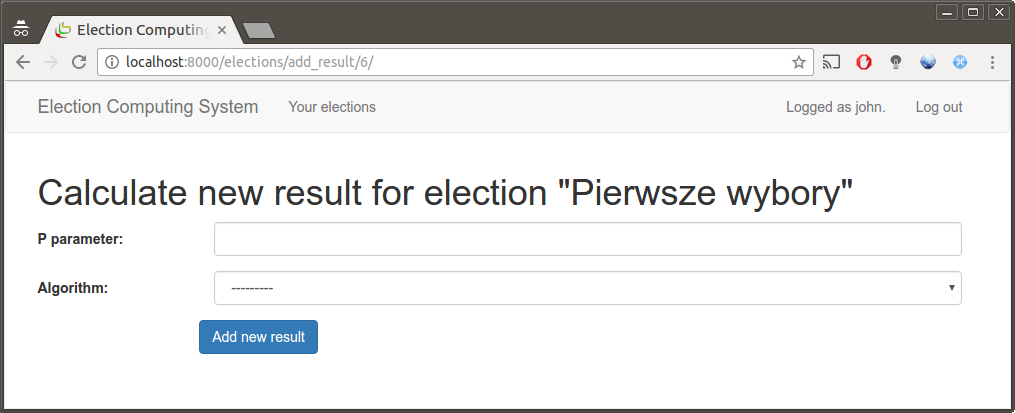
\includegraphics[width=0.8\textwidth]{pics/new-result.png}
\captionof{figure}{Strona z formularzem do określenia parametrów obliczania wyników wyborów}
\end{center}

\vspace{\baselineskip}
Wyświetlony formularz składa się z dwóch pól: parametru $p$ wpływającego na funkcję satysfakcji oraz typu algorytmu. Jako parametr $p$ można ustawić dowolną liczbę naturalną. Z kolei jako typ algorytmu można wybrać jedną z czterech możliwości: algorytm typu brute-force (\textit{Brute force}), algorytm genetyczny (\textit{Genetic}), algorytm zachłanny zależny od parametru $p$ (\textit{Greedy Algorithm}) oraz algorytm zachłanny według zasady \textit{Chamberlin-Courant’a} (\textit{Greedy CC}). Jeżeli zostanie wybrany algorytm inny od genetycznego, wtedy po wyborze tego typu algorytmu i parametru $p$, można rozpocząć obliczanie wyniku wyborów poprzez zatwierdzenie wyboru przyciskiem \textit{Add new result}. 

\newpage
Jeżeli jako typ algorytmu zostanie wybrany algorytm genetyczny, wtedy w formularzu wyświetlą się trzy dodatkowe pola do określenia parametrów algorytmu genetycznego: \\

\begin{center}
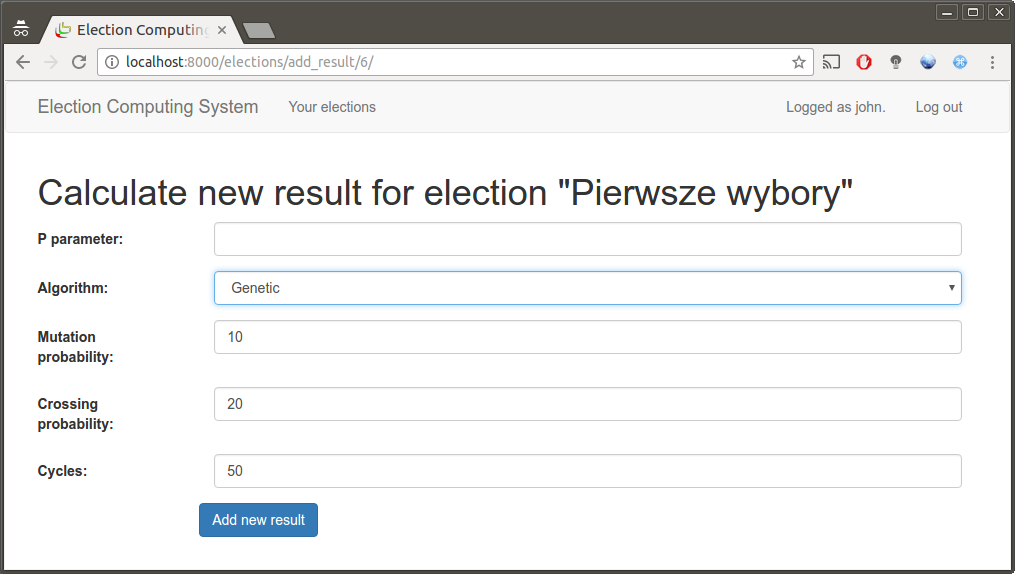
\includegraphics[width=0.8\textwidth]{pics/new-result-genetic.png}
\captionof{figure}{Strona z formularzem do określenia parametrów obliczania wyników wyborów algorytmem genetycznym}
\end{center}

\vspace{\baselineskip}
Dodane pola w formularzu począwszy od góry oznaczają odpowiednio: 
\begin{itemize}
\item prawdopodobieństwo wystąpienia mutacji w pojedynczym osobniku
\item część puli jaka jest poddawana krzyżowaniu
\item liczba cyklów działania algorytmu
\end{itemize}

Po określeniu wszystkich parametrów należy potwierdzić wybór przyciskiem \textit{Add new result}.
\newpage

\section{Szczegóły wyniku wyborów}
\label{sec:szczegolywyniku}

W celu wyświetlenia szczegółów wyników wyborów należy na stronie ze szczegółami wyborów nacisnąć odpowiednią ikonę danego wyniku wyborów w panelu z wynikami wyborów (\textit{Available results}): \\

\begin{center}
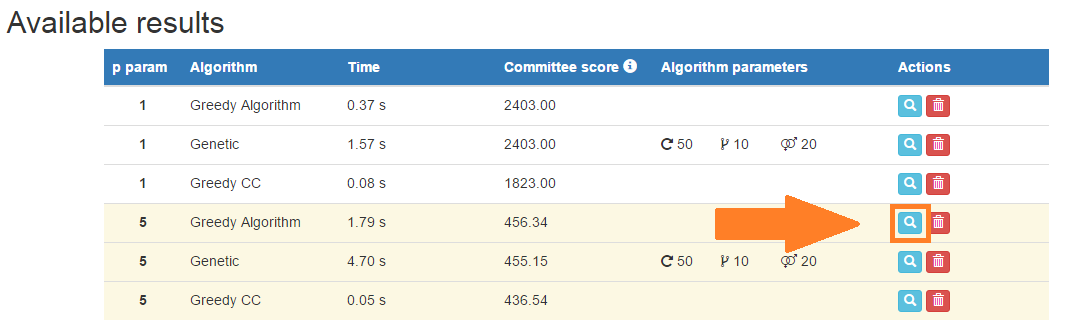
\includegraphics[width=0.8\textwidth]{pics/result_details_button.png}
\captionof{figure}{Przycisk kierujący do szczegółów danego wyniku wyborów}
\end{center} 

\vspace{\baselineskip}
Na stronie ze szczegółami wyników wyborów znajdują się wykres ze zwycięzcami (jeżeli wybory zostały wygenerowane z rozkładu normalnego) oraz lista zwycięzców: \\
\begin{center}
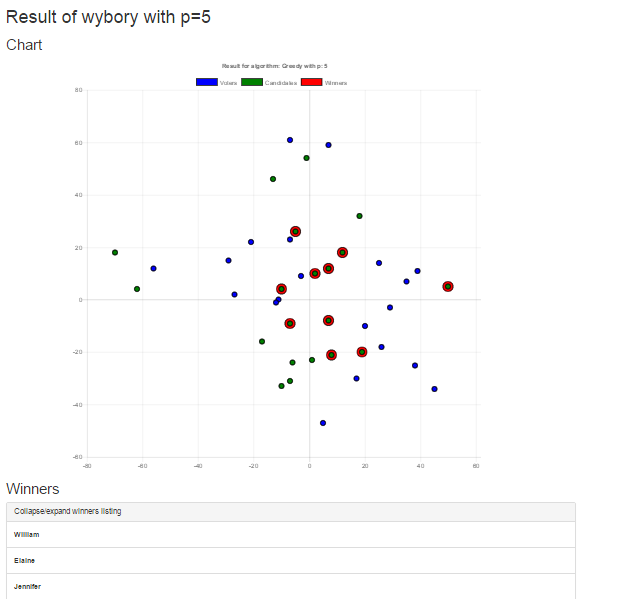
\includegraphics[width=0.8\textwidth]{pics/result-details_version2.png}
\captionof{figure}{Strona ze szczegółami wyników wyborów}
\end{center} 
%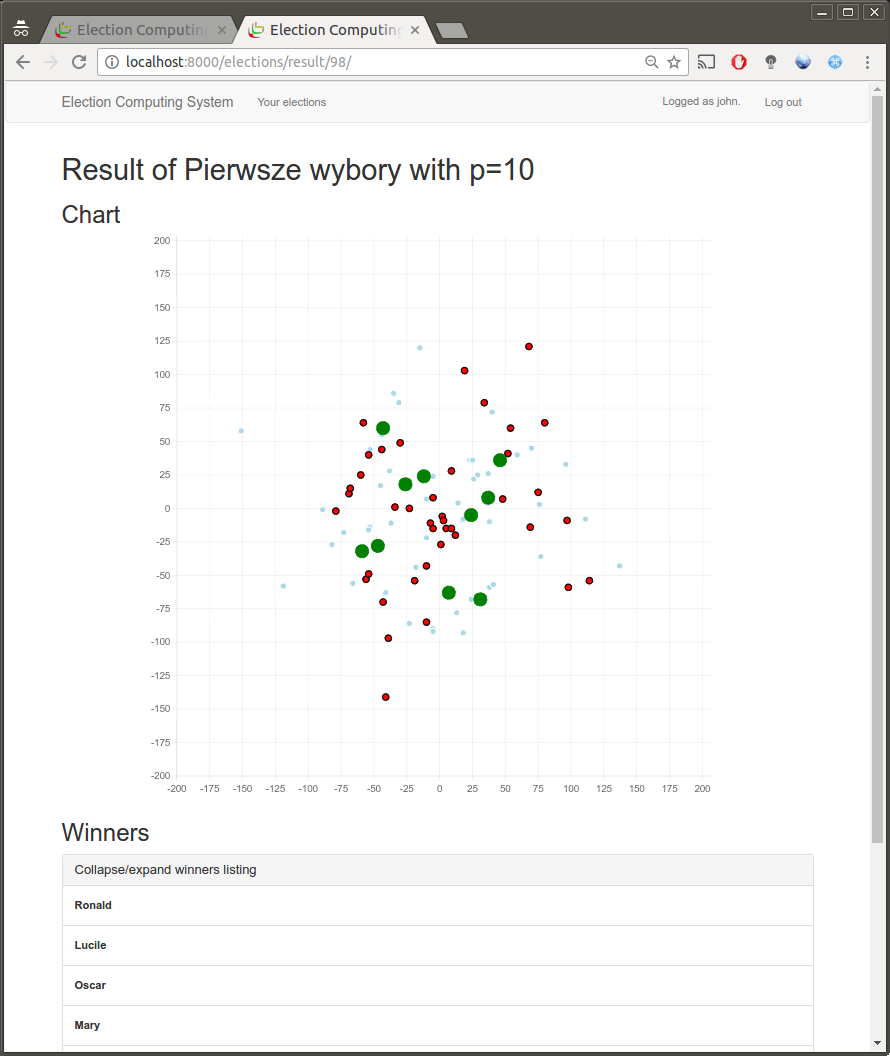
\includegraphics[width=0.8\textwidth]{pics/result-details.png}
\newpage

\section{Porównywanie wyników}
\label{sec:porownywaniewynikow}

\subsection{Używanie wykresu do porównywania wyników}
\label{subsec:pornawykresie}
Jednym ze sposobów porównywania wyników wyborów jest użycie na stronie ze szczegółami wyborów suwaka: \\

\begin{center}
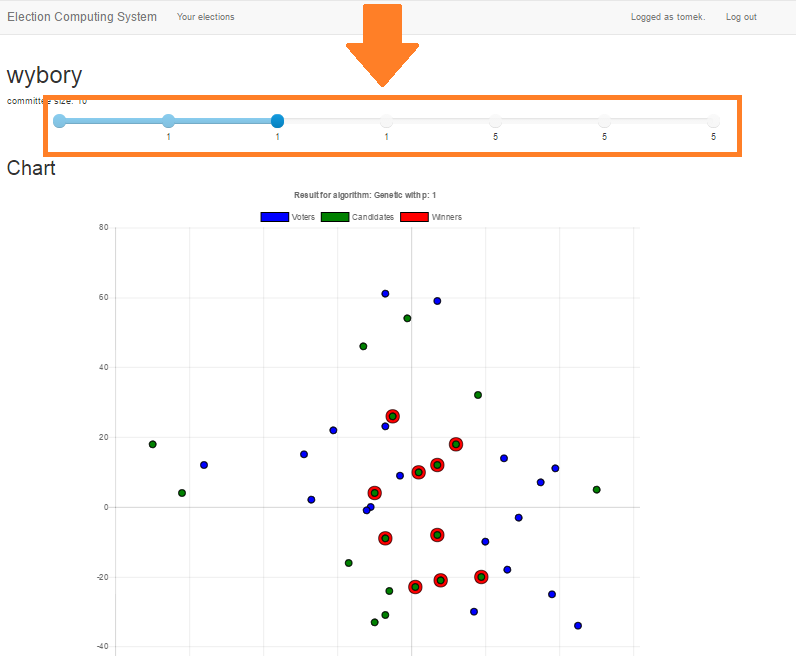
\includegraphics[width=0.8\textwidth]{pics/results_suwak.png}
\captionof{figure}{Suwak do porównywania wyników wyborów na stronie ze szczegółami wyborów}
\end{center}

\vspace{\baselineskip}
Suwak jest dostępny dla wyborów wygenerowanych z rozkładu normalnego. Suwak pozwala na porównywanie rozłożenia zwycięzców na wykresach dla różnych wartości parametrów $p$. Wykresy są takie same jak na stronach ze szczegółami wyników wyborów. 

\newpage
\subsection{Porównanie czasów wykonania obliczeń dla poszczególnych algorytmów}
\label{subsec:wykresczasuobliczen}

W sekcji \textit{Algorithms comparison} wyświetlany jest wykres zestawiający zależność czasu 
wykonania obliczeń od wartości parametru $p$ dla każdego algorytmu. Serie danych można ukryć lub 
wyświetlić klikając na etykiety z nazwami algorytmów znajdującymi się nad wykresem.

\begin{center}
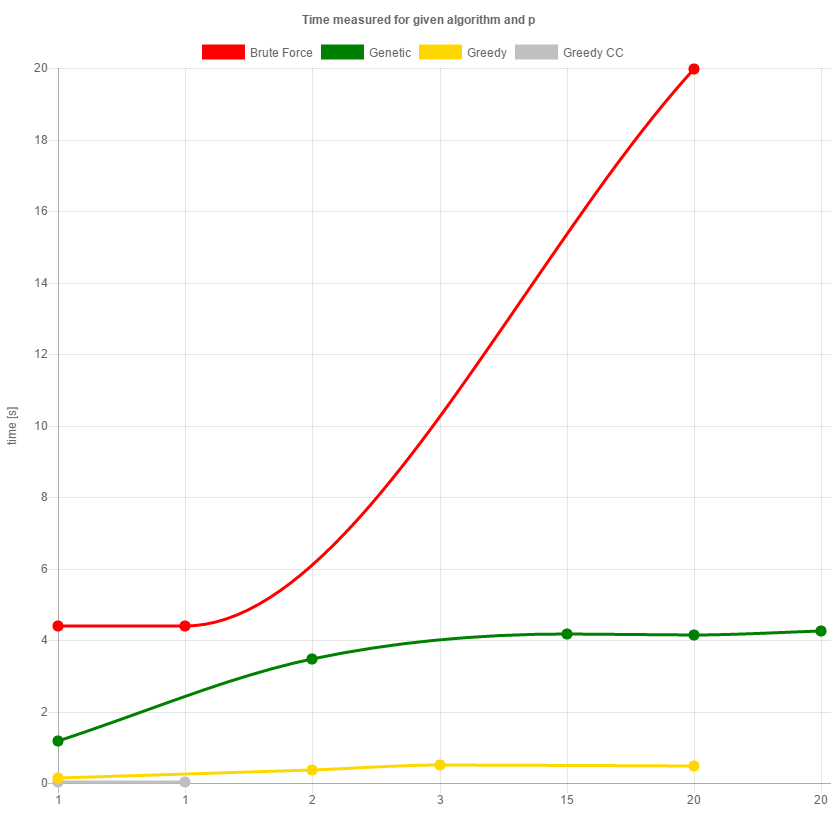
\includegraphics[width=0.6\textwidth]{pics/algorithms-comparison-1.png}
\captionof{figure}{Zestawienie czasów wykonania dla różnych algorytmów w zależności od parametru $p$}
\end{center}

\begin{center}
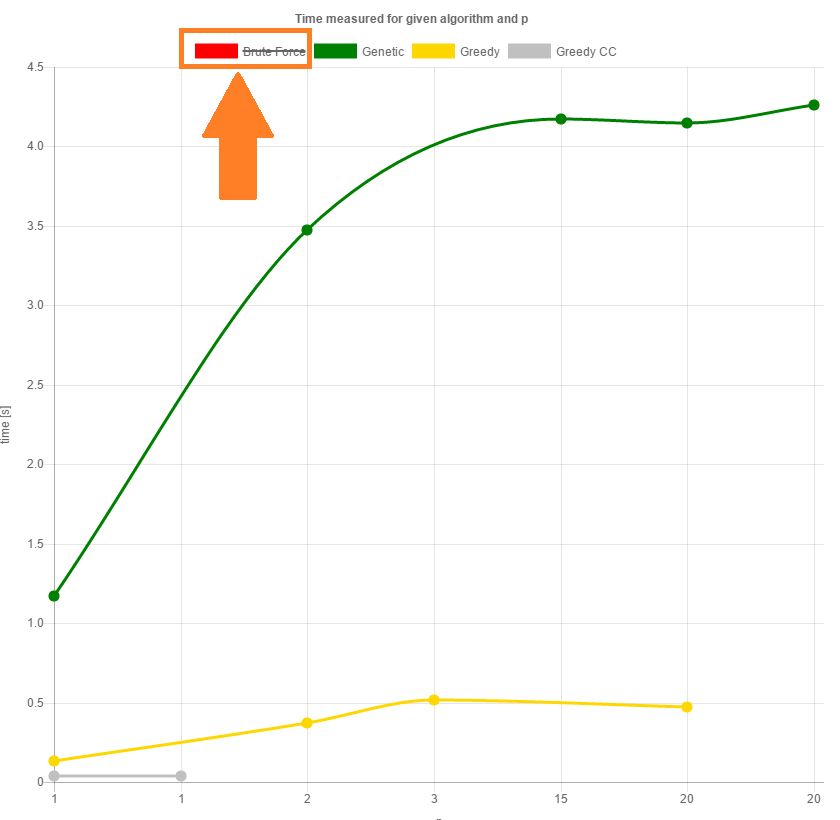
\includegraphics[width=0.6\textwidth]{pics/algorithms-comparison-2.png}
\captionof{figure}{Kliknięcie na etykietę danych z nazwą algorytmu powoduje ukrycie odpowiadającej mu 
serii danych}
\end{center}

\newpage
\subsection{Zestawienie wyników w tabeli}
\label{subsec:tabelazwynikami}

System umożliwia porównanie wyników wyborów na bazie zestawienia w tabeli czasów działania i jakości wyników wszystkich dostępnych rozstrzygnięć dla danych wyborów. Tabela znajduje się na stronie ze szczegółami wyborów w panelu \textit{Available results}: \\

\begin{center}
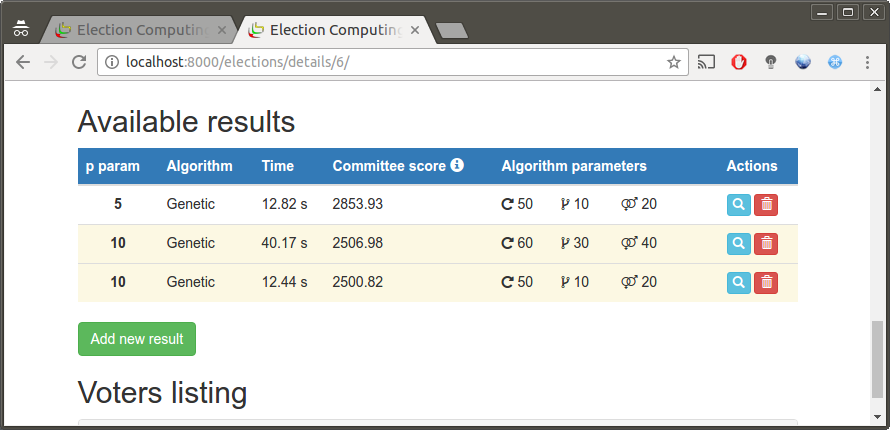
\includegraphics[width=0.8\textwidth]{pics/results-on-table.png}
\captionof{figure}{Zestawienie wszystkich wyników dla danych wyborów w postaci tabeli}
\end{center}

\section{Kasowanie wyników}
\label{sec:kasowaniewynikow}
W celu usunięcia danego wyniku wyborów należy na stronie ze szczegółami wyborami nacisnąć ikonę kosza przy danym wyniku wyborów: \\

\begin{center}
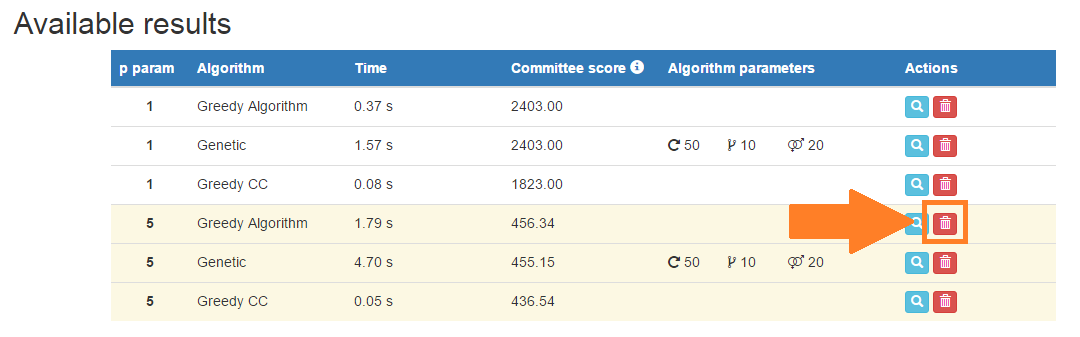
\includegraphics[width=0.8\textwidth]{pics/delete_result_button.png}
\captionof{figure}{Przycisk kierujący do formularza usuwania wyniku wyborów}
\end{center}

\newpage
Po naciśnięciu wskazanego przycisku pojawi się formularz, w którym należy potwierdzić chęć usunięcia danego wyniku wyborów: \\

\begin{center}
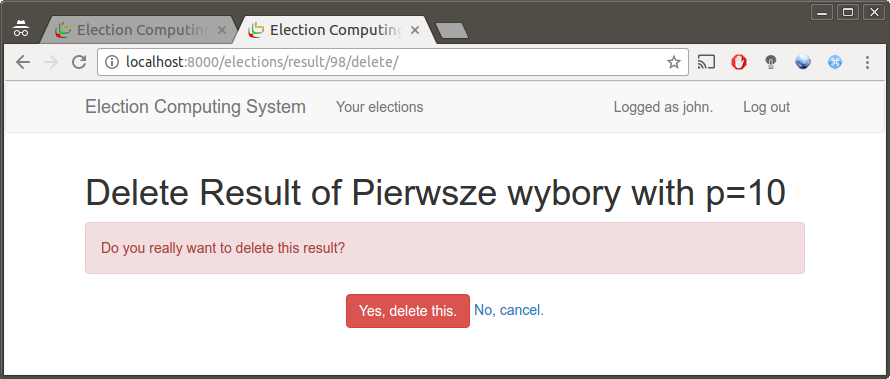
\includegraphics[width=0.8\textwidth]{pics/delete-result.png}
\captionof{figure}{Strona z formularzem do usuwania danego wyniku wyborów}
\end{center}

\vspace{\baselineskip}
W celu potwierdzenia chęci usunięcia danego wyniku wyborów należy nacisnąć przycisk \textit{Yes, delete this}.

\section{Kasowanie wyborów}
\label{sec:kasowaniewyborow}

W celu usunięcia danych wyborów należy na stronie z listą wszystkich wyborów nacisnąć ikonę kosza przy danych wyborach: \\

\begin{center}
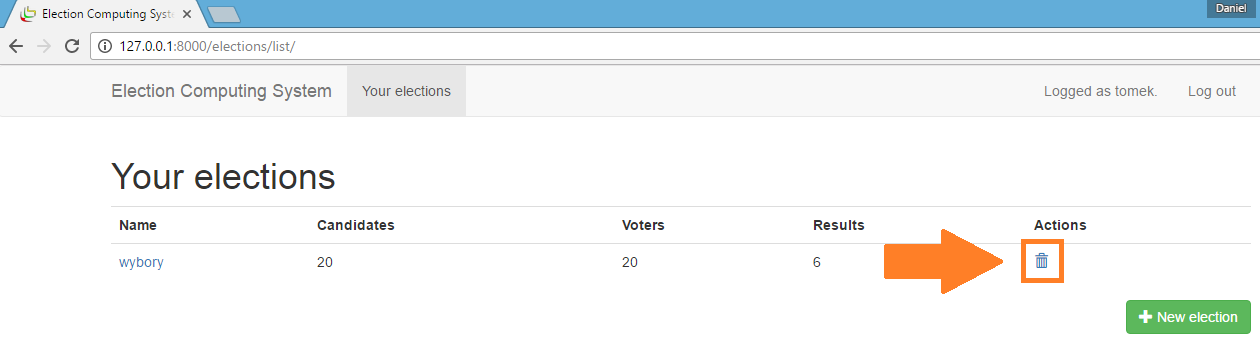
\includegraphics[width=0.8\textwidth]{pics/delete_election_button.png}
\captionof{figure}{Przycisk kierujący do formularza usuwania wyborów}
\end{center}

\newpage
Po naciśnięciu wskazanego przycisku pojawi się formularz, w którym należy potwierdzić chęć usunięcia danych wyborów: \\

\begin{center}
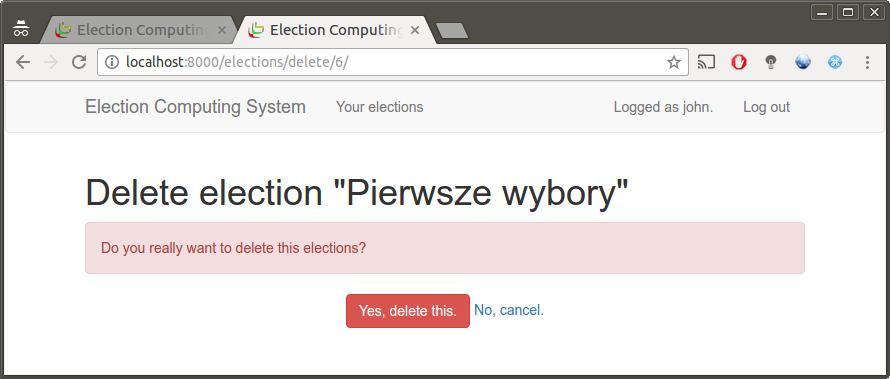
\includegraphics[width=0.8\textwidth]{pics/delete-elections.png}
\captionof{figure}{Strona z formularzem do usuwania danych wyborów}
\end{center}

\vspace{\baselineskip}
W celu potwierdzenia chęci usunięcia danych wyborów należy nacisnąć przycisk \textit{Yes, delete this}.

\chapter{Podsumowanie}
\label{cha:podsumowanie}

Twórcy systemu dążyli do zapewnienia dwóch podstawowych dogodności dla użytkowników. Pierwszą z nich była przystępna forma prezentacji wyników a drugą intuicyjna nawigacja po stronie.

\section{Prezentacja wyników}
Odpowiednia forma prezentacji wyników była sprawą nieodzowną dla dobrego działania systemu. Poza wymiarem estetycznym umożliwia zaobserwowanie sposobu zmieniania się wyników wyborów w zależności od parametrów przekazanych algorytmowi. W celu udogodnienia porównywania różnych wyników wyborów zaimplementowano suwak, który pozwala na proste przechodzenie między kolejnymi wykresami. W trakcie przechodzenia między wykresami punkty nie zmieniają swojego położenia na ekranie, dlatego wyraźnie widać każdą zmianę pomiędzy danymi wynikami wyborów.
 
\indent Innym udogodnieniem, które zostało wprowadzone jest sposób wyświetlania tabeli z czasami działania algorytmów oraz zadowoleniami jakie osiągnęły algorytmy. Poza estetyczną prezentacją tabeli, wyniki grupowane są według parametru p - wyniki dla tego samego parametru p są obok siebie. Ponadto tło grupy wyników jest pokolorowane w taki sposób, aby sąsiednie grupy miały inne tło. Dzięki takim zabiegom w prosty sposób można zlokalizować grupy wyników dla tego samego parametru p.

\section{Nawigacja po stronie}

Zarządzanie swoimi wyborami i ich wynikami było drugim aspektem, nad którym pochylili się twórcy aplikacji. Dążono do możliwie intuicyjnego interfejsu, który w łatwy sposób pozwoliłby na wykonywanie usług zapewnianych przez system. Przyciski zatwierdzające dane operacje odróżniają się od innych elementów strony przez co są łatwo widoczne. Ciąg operacji, które wykonuje użytkownik w celu wykonania danej akcji jest możliwie prosty i intuicyjny. Wyniki wyborów i same wybory są zgrupowane oddzielnie. Wyraźnie odróżnione są elementy klikalne i możliwe tylko do wyświetlenia.

\newpage
\cleardoublepage
\addcontentsline{toc}{chapter}{\listfigurename}
\listoffigures


\bibliographystyle{alpha}
\bibliography{bibliografia}

\end{document}
